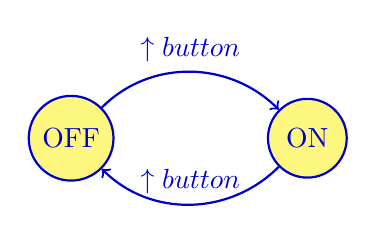
\begin{tikzpicture}

\def\colD{blue!80!black};
\def\colF{yellow!50!white};

\node[circle,thick,minimum size=1cm,
      draw=\colD,fill=\colF]
      (off) {\textcolor{\colD}{OFF}};

\node[circle,thick,minimum size=1cm,
      right of=off,node distance=3cm,
      draw=\colD,fill=\colF]
      (on) {\textcolor{\colD}{ON}};

\draw[->,thick,\colD]
      (off) to[out=45,in=135]
      node[pos=0.5,above]{$\uparrow button$}
      (on);

\draw[->,thick,\colD]
      (on) to[out=-135,in=-45]
      node[pos=0.5,above]{$\uparrow button$}
      (off);

\end{tikzpicture}